\documentclass{article}

\usepackage{amsthm}
\usepackage{amsmath}
\usepackage{graphicx}
\usepackage{verbatim}
\usepackage{amssymb}
\usepackage{float}

%\def\refname{Referinte}

\graphicspath{{res/}}

\newtheorem{fig}{Figure}[section]
\newtheorem{definition}{Definition}[section]
\newtheorem{prop}{Affirmation}[section]
\newtheorem{example}{Example}[section]
\newtheorem{explanado}{Explanation}[section]

%\renewcommand{\figurename}{Figura}

\begin{document}

\title{Logics and Deep Learning}
\author{Chris Luntraru}
\date{}
\maketitle

\begin{abstract}
This paper defines the ``Logic Tensor Network'' model, proposed by Luciano Serafini and Artur d'Avila Garcez to automate rationalization and learning on neural networks. A logic formalism called ``Real  Logic'' is defined based on a first order logic language, where formulas have truth values represented by real numbers within the interval [0, 1]. The Real Logic implemented in neural tensor networks allows deductive rationalization based on a knowledge base. These concepts are presented after a short introduction to neural networks and neural tensor networks. We then define real logic to be able to build the concept of Logic Tensor Networks.
\end{abstract}

\section{Introduction}
A number of kowledge bases like WordNet and Google Knowledge Graph are available today. They can be used for searching for certain data, the extraction of structured information made available to a user or even answering questions it has been asked. The increasing popularity of these services has garnered attention to research on the completion of knowledge bases. The idea is to implement a form of common knowledge, a simulation of human thinking when trying to deduce certain affirmations from incomplete knowledge. Humans are able to do this and it is a talent that we use every day. For example, if a person were to receive information that a new species of monkey was discovered, they would infer that this new monkey has arms, legs, maybe a tail, and so on. \cite{NTN} Recently, the machine learning industry has been seen to emphasize knowledge base completion, approximate deductions and rationalization based on statistics and neural networks. \cite{LTN}

\section{Neural Networks}
In order to understand more advanced concepts, such as Neural Tensor Networks and Logic Tensor Networks, it is necessary to have at least an intuitive image of the classic neural network used in Deep Learning. As such, a short presentation of this concept follows. Neural networks, are, as the name suggests, an imitation of the human nervous system. That being said, a component representative of the network is the neuron. \cite{Deep_Learning}

\begin{figure}[H]
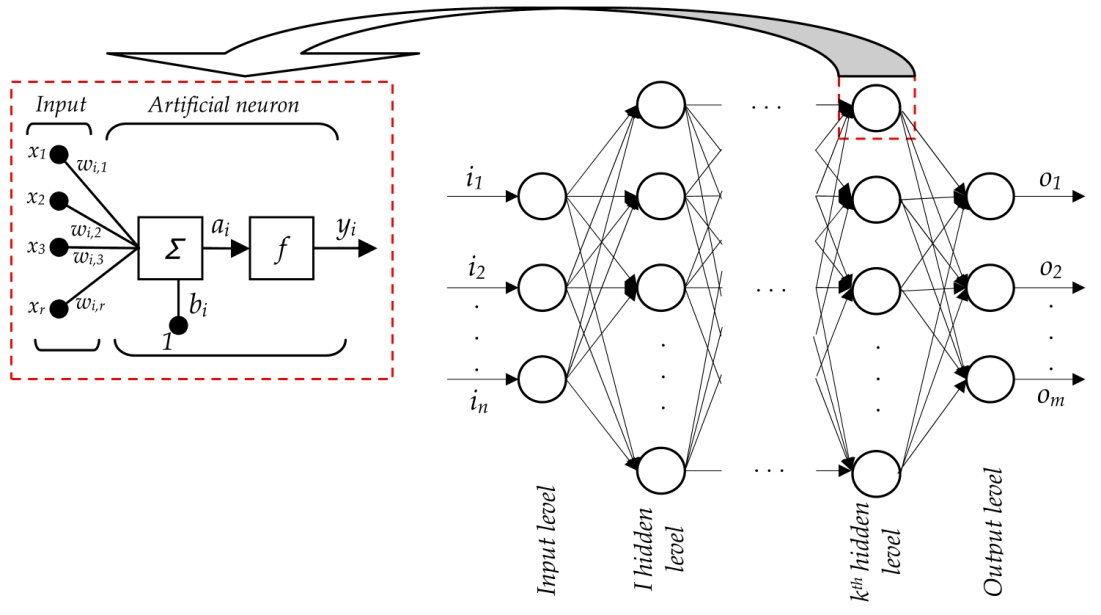
\includegraphics{ANN_Structure}
\caption{Neural network and neuron \cite{Deep_Learning}}
\end{figure}

A neural network is structured through layers. The first one is called the input layer and the last the output layer, while all of those in between are referred to as hidden layers. Their names reflect each of these layers' role in the network. The input layer does not compute anything, it just ``feeds'' a certain value to the first hidden layer, similar to the way hidden layers propagate information. The output layer, on the other hand, offers the user relevant information. The hidden layers are not literally ``hidden'', but the flow of information is humanly impossible to follow due to the immense number of nodes (neurons) and edges.

\subsection{Workings of a neuron}

\begin{figure}[H]
	\includegraphics[scale=0.5]{neuron_s}
	\caption{Neuron \cite{Deep_Learning}}
\end{figure}

Figure 1 illustrates the structure of an artificial neuron:\\

\begin{itemize}
	\item $x_1, x_2, ..., x_n$ are input. \\
	\item $w_0, w_1, w_2, ..., w_n$ are weights for each edge. \\
	\item $x0$ is the bias unit, and usuall has the value $+1$, $w_0$ being the one responsible for the bias effect on the end result.\\
	\item $a$ is the output of the activation function.\\
\end{itemize}

The output of an artificial neuron is calculated as follows:\\
$a = \sigma(\sum_{i=0}^n w_i x_i)$

\begin{example}
We can exemplify the functioning of a neural network by using simple calculations like the logical AND. The network's structure for the function is represented in Figure 3. In this case, the entire network is one single neuron, due to the simplistic nature of the calculation. The activation function, in this case, will be:\\
\[
	\sigma(x)= \left\{
	\begin{array}{ll}
	$0, if x $<$ 0$\\
	$1, if x $\geq$ 0$
	\end{array}
	\right.
\]\\
$x_1, x_2$ are inputs provided by the user and $b = -1.5$.\\
In this case, the output will be $a = \sigma(-1.5+x1+x2)$

\begin{figure}[H]
	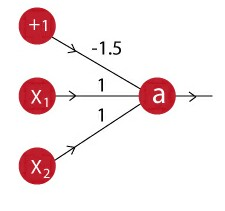
\includegraphics[scale=0.5]{and_s}
	\caption{Neural net for logical AND \cite{Deep_Learning}}
\end{figure}

\begin{figure}[H]
	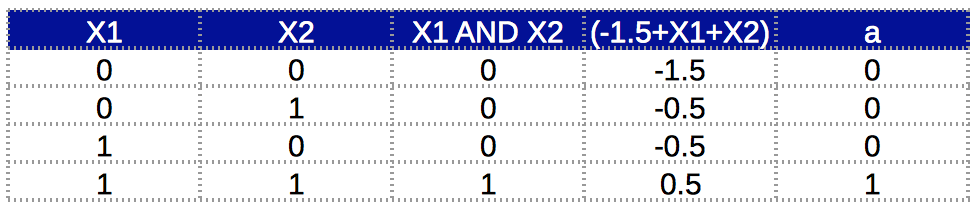
\includegraphics[scale=0.3]{and_table}
	\caption{Truth table for AND and $\sigma$ \cite{Deep_Learning}}
\end{figure}

\end{example}

\begin{example}
A more complex example, for which we need to use a larger number of nodes to create the network is the one for $\neg (x_1 \oplus x_2)$:\\
$\neg (x_1 \oplus x_2) = \neg((x_1+x_2) \land (\neg x_1 + \neg x_2))$

\begin{figure}[H]
	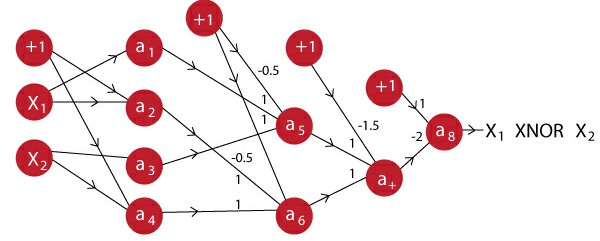
\includegraphics[scale=0.5]{xnor_s}
	\caption{Neural net for XNOR \cite{Deep_Learning}}
\end{figure}

\end{example}

\subsection{Backpropagation}
Understanding error minimization is imperative to gaining an accurate view of neural networks. In order to illustrate the concept, we study a relatively simple algorithm responsible for the error minimization of a neural network. It is called ``Backpropagation'' \cite{Deep_Learning}. In accordance with the name, the algorithm updates weights of edges babsed on the error reflected in the output layer. To gain an understanding of how the algorithm works, we need to define the partial derivative.

\begin{figure}[H]
	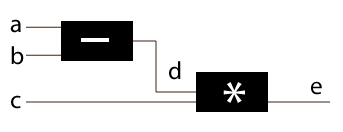
\includegraphics[scale=0.5]{gradient_diagram}
	\caption{Partial derivative in a neural net \cite{Deep_Learning}}
\end{figure}

\begin{definition}[Partial Derivative]
The partial derivative of a function with respect to a variable is the speed at which it changes for a change in the mentioned variable. \cite{Deep_Learning}\\
\end{definition}

\begin{example}
Figure 6 contains a simple neural network, for which we will compute the partial derivatives of the function $f(a, b, c) = (a - b) \cdot c$. We declare $d = a + b$ si $e = d \cdot c$:\\
$\cfrac{\partial e}{\partial d} = c$\ \ \ \ 
$\cfrac{\partial e}{\partial c} = d$\\ \\
$\cfrac{\partial d}{\partial a} = 1$\ \ \ \ 
$\cfrac{\partial d}{\partial b} = -1$\\ \\
To compute the partial derivatives with regards to a and b, we need to make use of simple algebric rules:\\
$\cfrac{\partial e}{\partial a} = \cfrac{\partial e}{\partial d} \cdot \cfrac{\partial d}{\partial a} = c$ \\ \\ 
$\cfrac{\partial e}{\partial b} = \cfrac{\partial e}{\partial d} \cdot \cfrac{\partial d}{\partial b} = -c$ \\
\end{example}

As a result, we know the effect that each node has on the output furnished by the network and we can begin to train the network.

\begin{definition}[Training]
Training a neural network refers to running it on a set of data for which an expected result is knows, and modifying the weights of edges by small values, in order to obtain a closer output to what is known to be corect.
\end{definition}

The weight of a variable $x$ is to be modified by a value based on the partial derivative of the network with regards to $x$ and the neuron's error.\\
The error of a neuron is calculated based on the error of the following layer.

\section{Tensor}
Tensors are an advanced mathematical concept that are a part of multilinear algebra. Though the aforementioned mathematical object conceptually extends far past the relevant scope in this paper, it is imperative  to at least conceptually grasp the notion before moving on to the Neural Tensor Network, the cornerstone behind Logic Tensor Networks.

\begin{definition}[Tensor]
An r-th rank tensor of order n is an n-dimensional mathematical object with $n^r$ components. \cite{Tensor}
\end{definition}

\begin{prop}
The order n of a tensor is the number of dimensions of the space it is defined in. \cite{Tensor}
\end{prop}

\begin{prop}
The rank r of a tensor is the number of directions it determines. \cite{Tensor_Rank}
\end{prop}

\begin{prop}
	Let $v_1$ and $v_2$ 1st-rank tensort of the 3rd order, such that they can be represented by tridimensional vectors:\\
	$v_1 = a_1 \cdot \vec{i} + b_1 \cdot \vec{j} + c_1 \cdot \vec{k}$\\
	$v_2 = a_2 \cdot \vec{i} + b_2 \cdot \vec{j} + c_2 \cdot \vec{k}$\\
	The product of these tensors \cite{Tensor_Multiplication} is calculated in a similar manner to the product of the polynomials that represent them, the result being a 2nd-rank tensor of the 3rd order:\\
\begin{align*}
	\overrightarrow{\overrightarrow{v_1 v_2}} = &a_1 a_2 \overrightarrow{\overrightarrow{ii}} + a_1 b_2 \overrightarrow{\overrightarrow{ij}} + a_1 c_2 \overrightarrow{\overrightarrow{ik}}\\
	&b_1 a_2 \overrightarrow{\overrightarrow{ji}} + b_1 b_2 \overrightarrow{\overrightarrow{jj}} + b_1 c_2 \overrightarrow{\overrightarrow{jk}}\\
	&c_1 a_2 \overrightarrow{\overrightarrow{ki}} + c_1 b_2 \overrightarrow{\overrightarrow{kj}} + c_1 c_2 \overrightarrow{\overrightarrow{kk}}\\
\end{align*}
where $\overrightarrow{\overrightarrow{ii}}, \overrightarrow{\overrightarrow{ij}},...,\overrightarrow{\overrightarrow{kk}}$ are 2nd-order unit tensors. The resulted tensor can be represented through the following matrix:\\
 \[
   M=
  \left[ {\begin{array}{ccc}
  	a_1 a_2	 & a_1 b_2 & a_1 c_2 \\
	b_1 a_2	 & b_1 b_2 & b_1 c_2 \\
	c_1 a_2	 & c_1 b_2 & c_1 c_2 \ 
  \end{array} } \right]
\]
\end{prop}

\begin{prop}
Tensor multiplication can be generalised. An rth-rank tensor of the nth order can be obtained through the multiplication of r tensors of the nth order.
\end{prop}

\section{Neural Tensor Networks}
The model is introduced in article \cite{NTN}. The authors mean to implement a form of common sense in neural networks, interpreted as the inference of certain relationships between objects, based on a set of data. In other words, the goal is to be able to determine if two entitied $e_1$ and $e_2$ are in a relationship R, given a certain knowledge base. To achieve this goal, the entities are represented as tensors to describe the respective objects. It adds to classic neural networks by providing a way to directly establish a relationship between objects, without simply concatenating the two entity vectors.

\begin{definition}[Neural Tensor Networks]
A neural tensor network is a neural networks that interprets objects received as input as nth-rank tensors of the 1st order.
\end{definition}

\begin{prop}
Since the tensors we consider are of the 1st order, they can be seen as vectors $v \in \mathbf{R}^n$. As a consequence, we can conveniently represent the numeric attributes of an object as coefficients on a certain dimension.
\end{prop}

\begin{example}
Let O be the set of people characterized by height, weight and sex. We measure height in cm, weight in kg and sex as a boolean value (0 being for male and 1 for female). In this case, a 1.8m tall man weighing 75kg can be represented as:\\
$v = <180, 75, 0> \in \mathbf{R}^3$
\end{example}

%\begin{figure}[H]
%	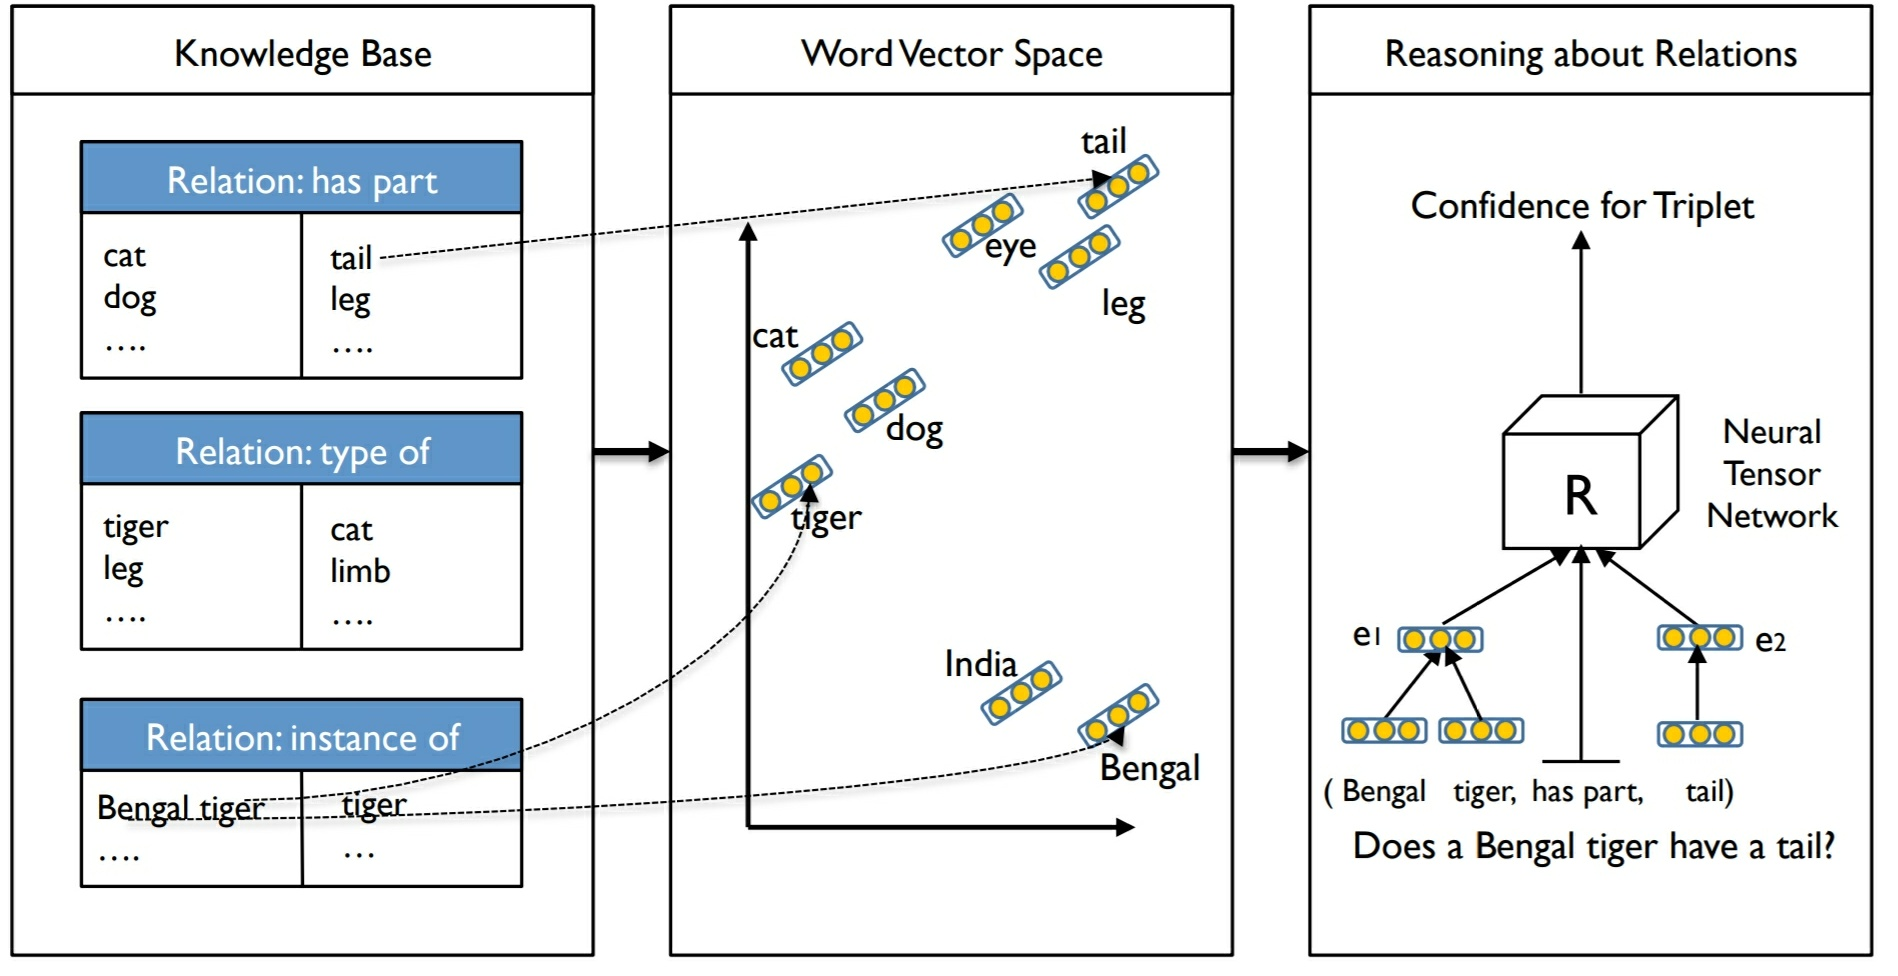
\includegraphics[scale=0.15]{NTN_graphical}
%	\caption{Graphical representation of a Neural Tensor Network's functionality \cite{NTN}}
%\end{figure}

The function that determines the probability that 2 entities are in a relationship has the following general form \cite{NTN}: \\ \\ 
$g(e_1, R, e_2) = U_R^T tanh(e_1^T W_R^{[1:k]}e_2 + V_R \left[\begin{smallmatrix} o_1 \\ o_2 \end{smallmatrix}\right] + b_R)$, where:\\
\begin{itemize}
	\item tanh = hyperbolic tangent, a standard nonlinearity
	\item k is the number of interpretations of the relationship R  (for example, two interpretations for the relation ``is a part of'' could be: ``foot'' is a part of ``dog'' or ``tire'' is a part of ``car'')
	\item $W_R^{[1:k]}$ is a tensor
	\item the product $e_1^T W_R^{[1:k]}e_2$ is the result of a k-dimensional vector of scalars that, computed through tanh and the other operations, will be in the interval [0, 1]
\end{itemize}

The other parameters are a part of the standard form of a neural network \cite{NTN}:\\
\begin{itemize}
	\item $e_1$ si $e_2$ the 2 objects for which we decide if they are in the relationship R
	\item d the number of dimensions of the vectors that represent $e_1$ si $e_2$
	\item $V_R \in \mathbf{R}^{k \cdot 2d}$, where $V_R \left[\begin{smallmatrix} o_1 \\ o_2 \end{smallmatrix}\right]$ establishes the relationship between $e_1$ and $e_2$ by concatenating the vectors (the ``classic'' approach)
	\item $U_R \in \mathbf{R}^k$ is to be multiplied with the k-dimensional vector to obtain a scalar, a real number in the interval [0, 1]
	\item $b_R \in \mathbf{R}^k$ the bias unit
\end{itemize}

\begin{figure}[H]
	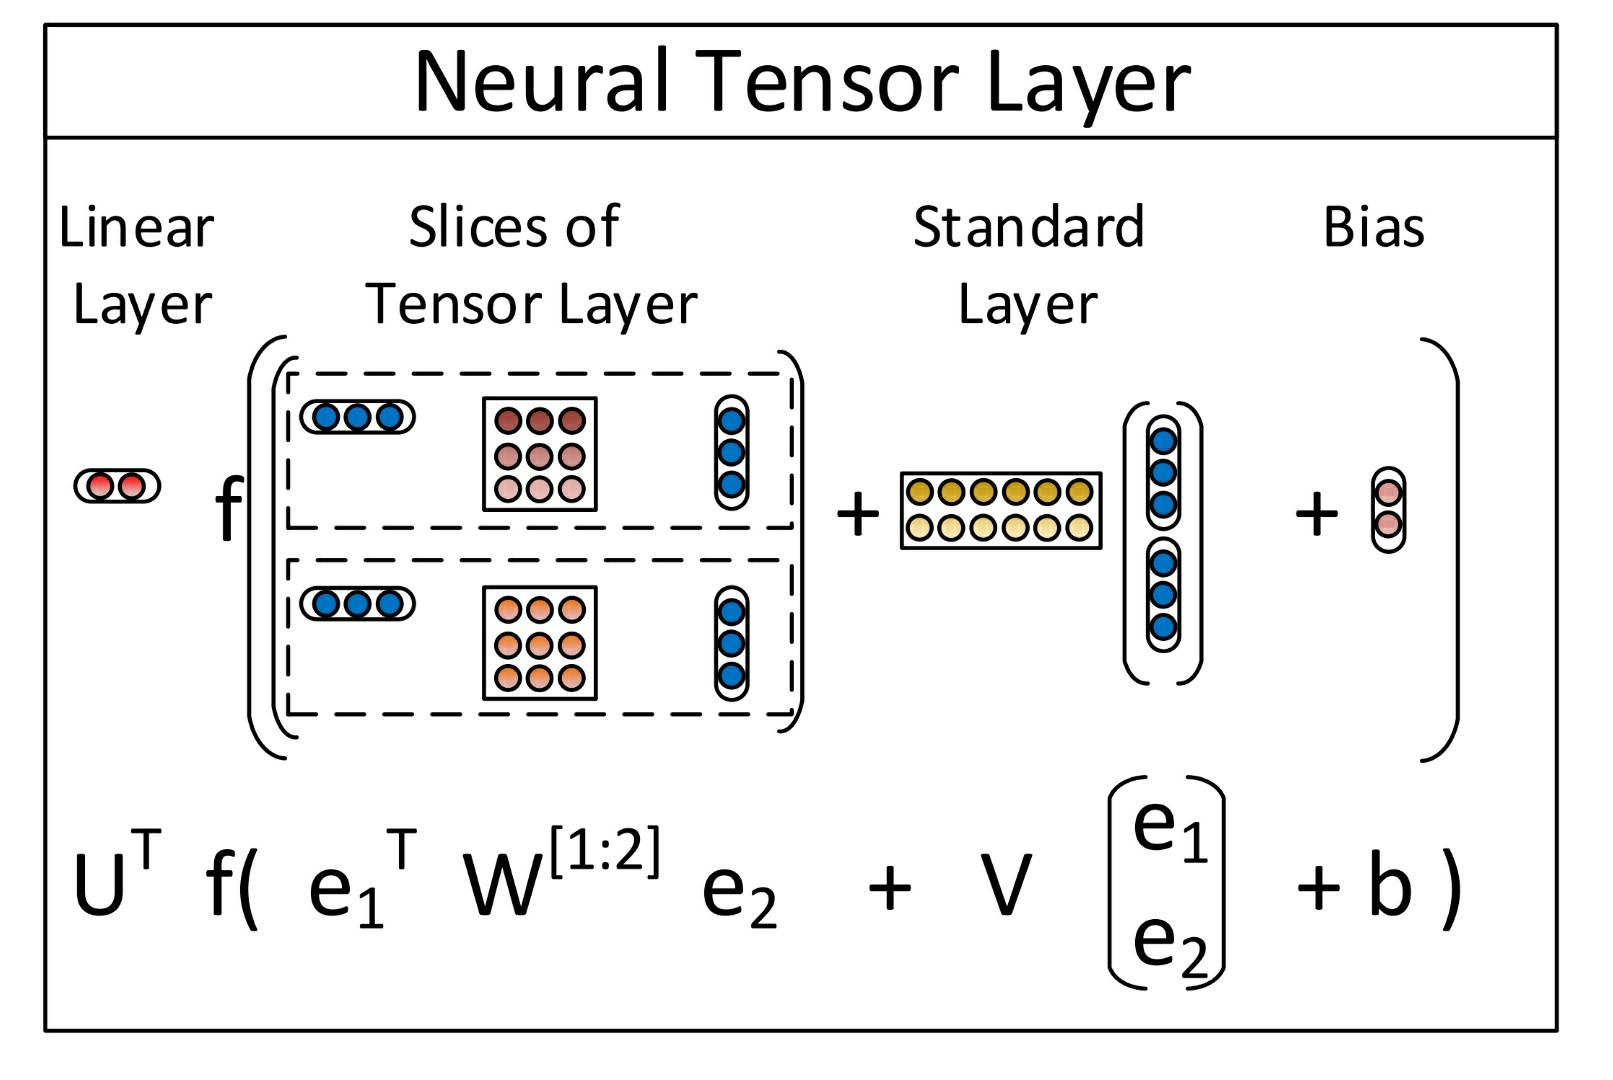
\includegraphics[scale=0.15]{ntn_rep}
	\caption{Graphical representation of the formula \cite{NTN}}
\end{figure}

\section{A short presentation of first order logic}
A number of elementary notions from first order logic are necessary to grasp the Logic Tensor Network. It is not necessary to present first order logic in detail and, as such, only concepts relevant to Real Logic will be defined.

\begin{prop}[The first order language]
The symbols of a first order language $\mathcal{L}$ are \cite{FOL}:\\
\begin{itemize} 
	\item a set of symbols for functions of specified arity
	\item a set of symbols for relationships, for example ``=''
	\item a set  of symbols for constants
	\item quantifiers like ``for all'' ($\forall$) and ``exists'' ($\exists$)
	\item an infinite set of variables $v_0, v_1, ..., v_n, \forall n \in \mathbf(N)$
	\item logical connectors, such as $\neg, \land, \lor$
	\item parantheses and the comma ``('', ``,'', ``)''
\end{itemize}
\end{prop}

\begin{definition}[Term]
A term t of a first order language $\mathcal{L}$ is a variable or constant of a language. \cite{FOL}
\end{definition}

\begin{definition}[Atom]
An atom is a formula with no deeper propositional structure. \cite{Atomic_Formula}
\end{definition}

\begin{definition}[Literal]
A literal is an atom or the negation of an atom. \cite{Literal}
\end{definition}

\begin{definition}[Clause]
A clause $\phi$ of a language $\mathcal{L}$ is an expression made up of a number of literals, true if any one of these literals is true. \cite{Clause}
\end{definition}

\begin{prop}
A clause $\phi$ is usually represented as:\\
	$\phi = \phi_1 \vee \phi_2 \vee ... \phi_k$, where $k \in \mathbf{N}$ is the number of literals that comprise it. \cite{Clause}
\end{prop}

\begin{definition}[Closed term/Closed clause]
A closed term/closed clause is a term/a clause that does not contain variables. \cite{Closed_Term}
\end{definition}

\begin{definition}[Free Variable]
A variable in a formula is free if it has no quantifier. \cite{Free_Variable}
\end{definition}

\begin{example}
In the formula $\forall yP(x, y)$, x is a free variable.\cite{Free_Variable}
\end{example}

\begin{example}
Let x and y variables and the functions:\\
friend(x, y) = x and y are friends\\
smoke(x) = x smokes\\
cancer(x) = x has cancer\\ \\
Then, the expression:\\
$\forall xy(friend(x,y) \land smoke(x)) \rightarrow smoke(y)$ \\
is read ``For all x and y such that x and y are friends and x smokes, y smokes.''
\end{example}

\section{Logic Tensor Network}
The goal of this model is to introduce an adequate way to implement learning an rationalization an integrate it into an idealized agent (for example, a self driving care). The agent needs to be able to work with information from a potentially infinite set of objects $\mathcal{O} = {o_1, o_2, ...}$. Thes objects are associated with a set of numeric attributes, through n-dimensional vectors (1st-rank tenors of the nth order). These tuples participate in a set of relationships $\mathcal{R} = {R_1, R_2, ..., R_k}$, where $R_i \subseteq \mathcal{O}^{\alpha(R_i)}$, where $\alpha(R_i)$ is the arity of the relationship $R_i$. Considered to be known are the following \cite{LTN}:\\
\begin{itemize}
	\item there exists a relationship between these numeric properties
	\item a network of relationships $\mathcal{R}$ in $\mathcal{O}$. 
\end{itemize}

Based on this incomplete knowledge, the agent must deduce the following  \cite{LTN}:\\
\begin{itemize}
	\item new information about the network of relationships among the objects of $\mathcal{O}$
	\item the numeric properties and classes of objects in $\mathcal{O}$
\end{itemize}
where the class of an object refers to the category it is a part of. For example, if we define the classes adult, child, person on the language $\mathcal{L}$, the expression $person(x) \wedge (adult(x) \vee child(x))$ has a truth value of 1. Most of the time, classes and relationships are not independent. More precisely, if an object x is of a class C ($C(x)$) and is in a relationship R with y, we can infer, in certain contexts, $C(y)$. The truth value of $C(y)$ depends on the situation. Therefore, we can deduce C(y) from training examples, but once we accumulate more knowledge it might be necessary to review this deduction. These ideas are implemented with the help of Neural Tensor Networks while using the power of first order logic to express affirmations.

The Logic Tensor Network introduced in the article \cite{LTN} is based on a new paradigm of logic, Real Logic.

\subsection{Real Logic}
We define real logic in order to be able to build upon the Neural Tensor Network \cite{NTN}. We define a set of new concepts, for example the grounding of a term and derived notions. These will be integrated into the NTN (\cite{NTN}) model and create a more effective means for knowledge base completion.

We start from a first order language $\mathcal{L}$ that contains \cite{LTN}:\\
\begin{itemize}
	\item $\mathcal{C}$ the set of constants
	\item $\mathcal{F}$ the set of functions
	\item $\mathcal{P}$ the set of predicates
\end{itemize}

The expressions in $\mathcal{L}$ have the goal of expressing relational knowledge \cite{LTN}:\\
\begin{example}
$R(o_1, o_2)$ states that $o_1 si o_2$ are in the relationship R\\
$\forall xyR(x, y) \rightarrow R(y, x)$ states that the relationship R is symmetrical\\
\end{example}

To emphasize the fact that $\mathcal{L}$ is interpreted in the real world, we define the concept of grounding \cite{LTN}:\\
\begin{itemize}
	\item The grounding $\mathcal{G}$ of a term t in the language $\mathcal{L}$ is an n-vector that represents the set of numeric attributes associated to it.\\
	\item The grounding $\mathcal{G}$ of a clause $\phi$ is a real number in the interval [0, 1] that represents the degree of confidence in the truth value of $\phi$.\\
\end{itemize}

\begin{prop}
All the constants c and variables v of a language $\mathcal{L}$ are terms. Moreover, any F(c) or F(v) is a term, while nothing else is considered to be a part of this category. \cite{FOL}
\end{prop}

\begin{definition}[Signature of a language]
The signature of a first order language $\mathcal{L}$ is $\mathcal{C} \cup \mathcal{F} \cup \mathcal{P}$. \cite{FOL}
\end{definition}

\begin{definition}[Instantiation]
The instantiation of a formula refers to replacing all the variables with constants. \cite{LTN}
\end{definition}

\begin{example}
A possible instantiation of the formula P(x) is P(2).
\end{example}

\begin{definition}[Grounding]
The grounding $\mathcal{G}$ of a first order language $\mathcal{L}$ is a function defined on $\mathcal{L}$ with values in $\mathbf{R}^n$, for an arbitrary n. \cite{LTN}
\begin{itemize}
	\item $\mathcal{G}(c) \in \mathbf{R}^n, \forall c \in \mathcal{C}$
	\item $\mathcal{G}(f): \mathbf{R}^{n \cdot \alpha (f)} \rightarrow \mathbf{R}^n, \forall f \in \mathcal{F}$
	\item $\mathcal{G}(P): \mathbf{R}^{n \cdot \alpha (P)} \rightarrow [0, 1], \forall P \in \mathcal{P}$
\end{itemize}
\end{definition}

A grounding $\mathcal{G}$ can be inductively extended to all the terms of an expression \cite{LTN}:\\
\begin{itemize}
	\item $\mathcal{G}(f(t_1, t_2, ..., t_m)) = \mathcal{G}(f)(\mathcal{G}(t_1), \mathcal{G}(t_2), ..., \mathcal{G}(t_m))$, where $m = \alpha(f)$
	\item $\mathcal{G}(P(t_1, t_2, ..., t_m)) = \mathcal{G}(P)(\mathcal{G}(t_1), \mathcal{G}(t_2), ..., \mathcal{G}(t_m))$, where$m =\alpha(P)$
	\item $\mathcal{G}(\neg P(t_1, t_2, ..., t_m)) = 1 - \mathcal{G}(P(t_1, t_2, ..., t_m))$
	\item $\mathcal{G}(\phi_1, \phi_2, ..., \phi_k) = \mu(\mathcal{G}(\phi_1), \mathcal{G}(\phi_2), ..., \mathcal{G}(\phi_k))$, where k is the number of literals that form the clause $\phi$ and $\mu$ is a standard function for this kind of situation (a popular example would be $\mu_{max}(x, y) = max(x, y))$
\end{itemize}

\begin{explanado}
These rules define a grounding for any formula. Let n be the number of dimensions of a term $t_i, \forall i = \overline{1,  m}$. As a consequence, the tuple $ \langle \mathcal{G}(t_1), \mathcal{G}(t_2), ..., \mathcal{G}(t_m) \rangle$ is an ordered set of m n-dimensional vectors. The tuple contains $n \cdot m$ scalars, corresponding to the set f is defined on ($\mathbf{R}^{n \cdot \alpha(f)}$). The result is the grounding of a single term $v \in \mathbf{R}^n$. Analogously, we can follow the form of $\mathcal{G}(P)$. When referring to a clause $\phi$ we have: $\mathcal{G}(\phi) = \mathcal{G}(\phi_1 \vee \phi_2 \vee ... \phi_k) = \mu(\mathcal{G}(\phi_1), \mathcal{G}(\phi_2), ..., \mathcal{G}(\phi_k))$, where $\mathcal{G}(\phi_i) \in [0, 1], \forall i = \overline{1, k}$. \cite{LTN} 
\end{explanado}

\begin{example}
Let $\mathcal{O} = {o_1,o_2, o_3}$ be the set of documents defined on a finitie dictionary $D = {w_1, w_2, ..., w_n}$ of n words. Let $\mathcal{L}$ be the language that contains the binary function $concat(x, y)$  that denotes the document obtained by concatenating the two documents $x$ and $y$. Let $sim(x, y)$ be the binary predicate which is true is x and y are considered similar. In this case, we will use the cosine similarity function to decide that. As such, a relevant grounding of a document, in this case, would be the vector that denotes the number of apparitions of each word present in the dictionary. We define \cite{LTN}:\\
\begin{itemize}
	\item $\mathcal{G}\langle n_{w_1}^{o_i}, n_{w_2}^{o_i}, ... n_{w_n}^{o_i}\rangle$, where $n_{w}^{o}$ is the number of apparitions of word w in document o
	\item Let $u, v \in \mathbf{R}^n$ be the groundings of 2 arbitrary documents in $\mathcal{O}$. Then, $\mathcal{G}(concat)(u, v) = u + v$
	\item Let $u, v \in \mathbf{R}^n$ be the groundings of 2 arbitrary documents in $\mathcal{O}$. Then, $\mathcal{G}(sim)(u, v) = \frac{u \cdot v}{||u|| \cdot ||v||} =\cos(\theta)$, where $\theta$ is the angle between u and v
\end{itemize}

More precisely if the 3 documents and the dictionary are:\\
\begin{itemize}
	\item $o_1 = $``John studies logic and plays football''
	\item $o_2 = $``Mary plays football and logic games''
	\item $o_3 = $``John and Mary play football and study logic together''
	\item D = \{John, Mary, and, football, game, logic, play, study, together\}
\end{itemize}
then:\\
\begin{itemize}
	\item $\mathcal{G}(o_1) = \langle 1, 0, 1, 1, 0, 1, 1, 1, 0 \rangle$
	\item $\mathcal{G}(o_2) = \langle 0, 1, 1, 1, 1, 1, 1, 0, 0 \rangle$
	\item $\mathcal{G}(o_3) = \langle 1, 1, 2, 1, 0, 1, 1, 1, 1 \rangle$
	\item $\mathcal{G}(concat(o_1, o_2)) = \mathcal{G}(o_1) + \mathcal{G}(o_2) = \langle 1, 1, 2, 2, 1, 2, 2, 1, 0 \rangle$
	\item $\mathcal{G}(sim(concat(o_1, o_2), o_3)) = \frac{\mathcal{G}(concat(o_1, o_2)) \cdot \mathcal{G}(o_3)}{||\mathcal{G}(concat(o_1, o_2))|| \cdot ||\mathcal{G}(o_3)||} \approx  0.88$
	\item $\mathcal{G}(sim(o_1, o_3) \vee sim(o_2, o_3)) = \mu_{max}(\mathcal{G}(sim(o_1, o_3)), \mathcal{G}(sim(o_2, o_3))) =  \\
					=\mu_{max}(\mathcal{G}(sim)(\mathcal{G}(o_1), \mathcal{G}(o_3)), \mathcal{G}(sim)(\mathcal{G}(o_2), \mathcal{G}(o_3))) = \\
					= max(\cos(\mathcal{G}(o_1), \mathcal{G}(o_2)), \cos(\mathcal{G}(o_2), \mathcal{G}(o_3))) = \\
					= max(0.86, 0.73) = \\
					= 0.86$
\end{itemize}

\end{example}

Now that the grounding of a term has been established to be a representation of the real world counterpart of an object, we move on to concepts that are based on it, to further build the foundation of Logic Tensor Networks.

\subsection{Learning as approximate satisfiability}
We define satisfiability, partial groundings and grounded theory. These are what will be used to establish a confidence score for a clause, the real number in the interval [0, 1] used to determine whether an expression is to be considered true or not. 

\begin{definition}[Satisfiability]
Let $\phi$ be a closed clause in $\mathcal{L}$, $\mathcal{G}$ a grounding and $v \leq w \in [0, 1]$. We say that $\mathcal{G}$ satisfies $\phi$ in the confidence interval $[v, w]$ ($\mathcal{G} \models_v^w \phi$) if $v \leq \mathcal{G}(\phi) \leq w$. \cite{LTN}
\end{definition}

\begin{definition}[Partial grounding]
A partial grounding $\widehat{\mathcal{G}}$ is a grounding defined on a subset of the signature of the language $\mathcal{L}$. \cite{LTN}
\end{definition}

\begin{definition}[Grounded theory]
A grounded theory is a pair $\langle \mathcal{K},  \widehat{\mathcal{G}} \rangle$, where $\mathcal{K}	$ is a set of pairs $\langle [v, w], \phi(x) \rangle$, where $\phi(x)$ is a clause in $\mathcal{L}$ that contains the set x of free variables, $[v, w] \subseteq [0, 1]$ an interval and $\widehat{\mathcal{G}}$ is a partial grounding. \cite{LTN}
\end{definition}

\begin{explanado}
Intuitively, we can see a grounded theory $\langle \mathcal{K},  \widehat{\mathcal{G}} \rangle$ as the set $\mathcal{K}$ of clauses on which the partial grounding $\widehat{\mathcal{G}}$ is defined. \cite{LTN}
\end{explanado}

\begin{definition}[Satisfiability of a grounded theory]
A grounded theory $\langle \mathcal{K},  \widehat{\mathcal{G}} \rangle$ is satisfiable if
 $\exists \mathcal{G} \supseteq \widehat{\mathcal{G}}$ such that $\forall \langle [v, w], \phi(x) \in \mathcal{K} \rangle$ and any tuple t of closed terms $\mathcal{G} \models_v^w \phi(t)$. \cite{LTN}
\end{definition}

\begin{explanado}
In other words, a grounded theory is satisfiable if there exists a $\mathcal{G} \supseteq \widehat{\mathcal{G}}$ such that $\mathcal{G}$ satisfies all the clauses in $\mathcal{K}$ in the associated confidence intervals. \cite{LTN}
\end{explanado}

Based on this last definition, we arrive at the conclusion that, to determine whether a grounded theory $\langle \mathcal{K},  \widehat{\mathcal{G}} \rangle$ is satisfiable we would need to search for a $\mathcal{G} \supseteq \widehat{\mathcal{G}}$ in the set of all possible groundings, such that all instantiations of a clause in $\mathcal{K}$ are satisfiable with regards to the associated interval. Obviously, a similar approach would not be feasible. To obtain an algorithm that can be applied in practice, we notice that the number of instantiations of a clause in enormous, potentially infinite (for example when it contains a literal similar to $f(f(f(....f(x))))$), due to the fact that the language $\mathcal{L}$ permits the use of function symbols. Based on this observation, we can drastically reduce the time needed for instantiation by imposing a maximum depth to the operation (more precisely, in the abovementioned example, if we were to restrict the instantiation to a depth of 3, the literal would only be able to take the values $f(f(x_1)), f(f(x_2)), ...$). Furthermore, to avoid searching for a viable element in the set of all possible groundings, we will search for them in a certain class of functions, based on the fact that a grounding should establish a relationship between the numeric attributes of an object and the relationships it is in with other objects. \cite{LTN}\\ 
When a grounded theory $\langle \mathcal{K},  \widehat{\mathcal{G}} \rangle$ has no grounding $\mathcal{G}$ that satisfies it, we search for a grounding $\mathcal{G}$ that satisfies as much as possible out of $\langle \mathcal{K},  \widehat{\mathcal{G}} \rangle$. In other words, we need to find a grounding $\mathcal{G}$ that minimizes the satisfiability error, defined as follows:

\begin{definition}[Satisfiability error  of a grounded theory]
$Loss(\mathcal{G}, \langle [v, w], \phi \rangle) = min(|x - \mathcal{G}(\phi)|)$, where $x$ takes all the values in the interval $[v, w]$. \cite{LTN}
\end{definition}

\begin{prop}
If the value $\mathcal{G}(\phi)$ is in the interval $[v, w]$ given by $\mathcal{K}$, then $Loss(\mathcal{G}, \langle [v, w], \phi \rangle) = 0$. \cite{LTN}
\end{prop}

\begin{definition}[Approximate satisfiability]
Let $\langle \mathcal{K},  \widehat{\mathcal{G}} \rangle$ be a grounded theory and $\mathcal{K}_0$ a finite subset of the instantiations of the clauses in $\mathcal{K}$. Let $\mathbf{G}$ be a famiy of groundings. We define the problem of optimal satisfiability as finding a $\mathcal{G}^* \supseteq \widehat{\mathcal{G}}$ in $\mathbf{G}$ that minimizes the satisfiability error in $\mathcal{K}_0$. \cite{LTN}
\end{definition}

\begin{explanado}
Mathematically:\\
$\mathcal{K}_0 \subseteq \{ \langle [v, w], \phi(t) \rangle | \langle [v, w], \phi(x) \rangle \in \mathcal{K}$ si t este un n-tuplu de termeni inchisi\}\\ \\
$\mathcal{G}^* = \underset{\widehat{\mathcal{G}} \subseteq \mathcal{G} \in \mathbf{G}}{\operatorname{argmin}} \ \  \underset{\langle [v, w], \phi(t) \rangle}{\sum} Loss(\mathcal{G}, \langle[v, w], \phi(t) \rangle)$  \\ \\ so $\mathcal{G}^*$ is the value of $\mathcal{G}$ in which the sum of all satisfiability errors of clauses in $\mathcal{K}$ is the lowest possible number.
\end{explanado}

\section{Real Logic in Neural Tensor Networks}	
Let $\mathbf{G}$ be the space of tensor transformations of order k (where k is a parameter). In this space, functions are interpreted as linear transformations. The grounding of a predicate $P$ with arity m, $\mathcal{G}(P): \mathbf{R}^{mn} \rightarrow [0, 1]$ is defined as the generalisation of a neural tensor network \cite{NTN}: \\ \\
$\mathcal{G}(P) = \sigma (U_P^T \tanh(v^T W_P^{[1:K]} v + V_P v + B_p)$\\ \\
where the formula has the same explanation as with Neural Tensor Networks. By this interpretation, the truth value of a  clause can be determined  by a neural network that first calculates the grounding of the literals in the clause, then combines them using the specific function $\mu$. Figure 8 illustrates a tensor network for the expression $\neg P(x, y) \rightarrow A(y)$. In this case, the parameters $W_*, V_*, B_*$ and $U_*$, where $* \in \{P, A\}$ will be deduced as a result of training the network (maximizing the satisfiability of the clause). \cite{LTN}

\begin{figure}
	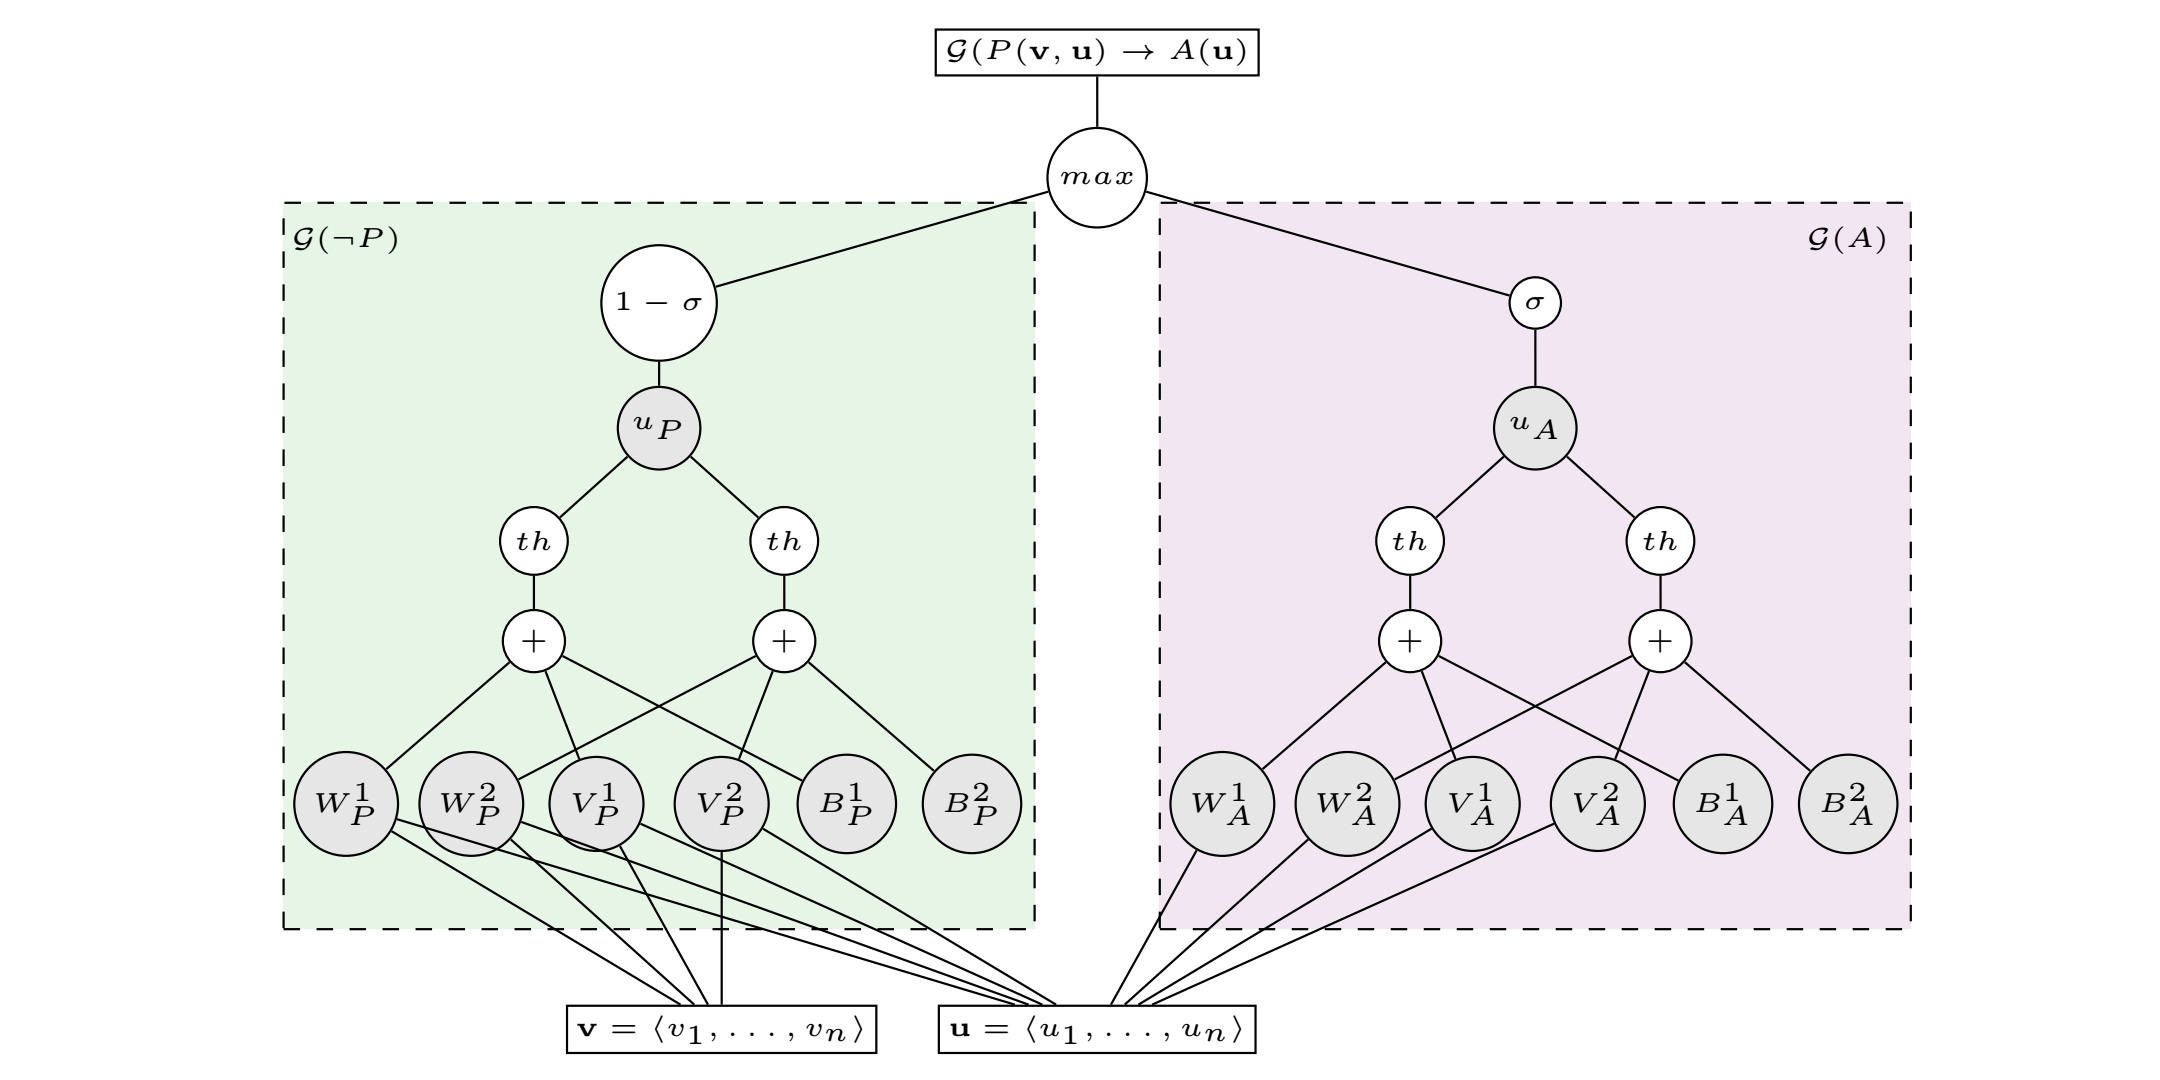
\includegraphics[scale=0.2]{ltn_exp}
	\caption{Tensor network for $\neg P(x, y) \rightarrow A(y)$, where $\mathcal{G}(x) = v$, $\mathcal{G}(y) = u$ si $k = 2$ \cite{LTN}}
\end{figure}

\section{An example of knowledge base completion}
Logic Tensor Networks have been implemented as a Python library named ``ltn'', using Google's TensorFlow. To illustrate the model's effectiveness, the authors make use of the well-known ``Friends and smokers'' example. Let there be 14 people separated into 2 groups: $\{ a, b, ..., h\}$ si $\{ i, j, ..., n \}$. In each group, we know who is a smoker and who isn't, while in the first group we also know who does and doesn't have cancer. We also have general information about smoking, friendship and cancer: smoking causes cancer, friendship is a symmetric and antireflexive (one cannot be friend with oneself) relatonship, everyone has at least one friend and smoking propagates among friends. All this information is represented in the knowledge base in Figure 9. The expressions, on the other hand, have different truth values, but that is not a known fact. If this weren't true, the resulting knowledge base would be inconsistent (it could, for instance deduce both $S(b)$ and $\neg S(b)$). The goal of the network is to: find the truth values of expressions in the knowledge base and find truth values for missing affirmations (like C(i)), but also find a suitable grounding for each constant $a, b, ...n$. To respond to these requests, ``ltn'' is used to approximate a complete knowledge base. We assume that all affirmations in the knowledge base are true (have a truth value of 1). To demonstrate the necessity of background knowledge, 2 experiments are followed: $\mathcal{K}_{exp1} = \mathcal{K}_{a...h}^{SFC} \cup \mathcal{K}_{i...n}^{SFC}$. In the second experiment ($exp2$) we introduce background knowledge, so: $\mathcal{K}_{exp2} = \mathcal{K}_{exp1} \cup \mathcal{K}^{SFC}$.\\
It is also necessary to configure the network: each constant (person) can have up to 30 real number attributes. The number $k$ of layers in the tensor network is 10 and the functiun $\mu$ used is $\mu(a, b) = min(1, a + b)$. An approximation of the ideal grounding is obtained after 5000 runs of the training algorithm RMSProp available in TensorFlow. The results of the 2 experiments are visible in the tables represented in Figure 10, where truth values above 0.5 are written in bold for legibility. The values are also colored the same as the knowledge base they originate from, while the inferred ones have a white background. To evaluate the quality of the results it is necessary to verify if the truth values of the information taken from the original knowledge bases are close to 1 and if the inferred knowledge corresponds to expectations.\\
It can be seen that the Logic Tensor Network associcated with $\mathcal{K}_{exp1}$ produces the same results as $\mathcal{K}_{exp1}$ itself, so the network produces expected results. Moreover, it infers additional information about $F$ and $C$ that cannot be derived from $\mathcal{K}_{exp1}$ through purely logical rationalization, for instance: $F(c, b)$, $F(g, b)$, $\neg F(b, a)$. These result from the similarity of the groundings of these constants, generated by the network. Specifically, $\mathcal{G}(c)$ and $\mathcal{G}(g)$ have a high cosine similarity (the rationale behind this is similar to the one behind the example based on the similarity between documents).\\

\begin{figure}[H]
	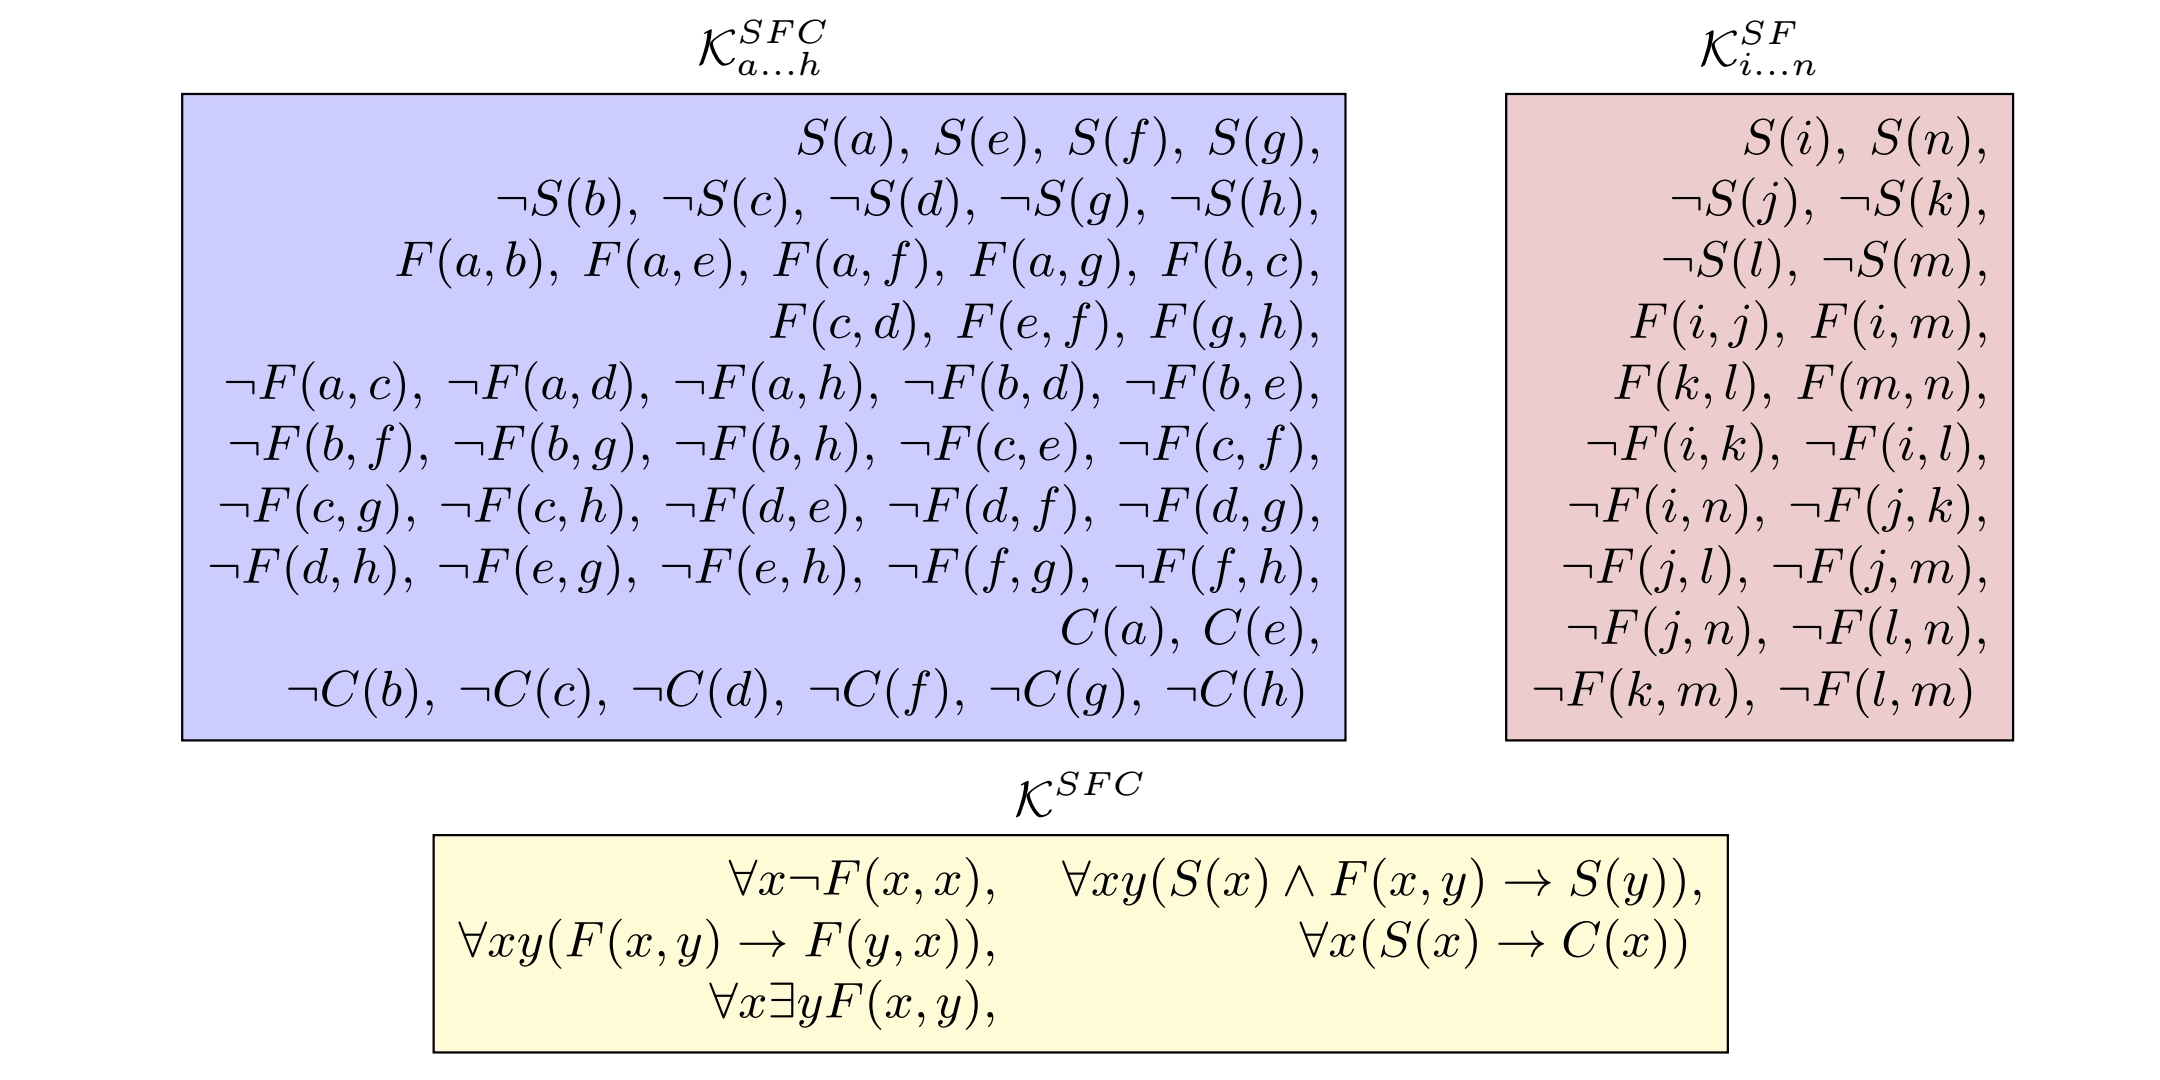
\includegraphics[scale=0.2]{kb}
	\caption{Initial knowledge base \cite{LTN}}
\end{figure}

The results of the second experiment prove that even more information can be deduced once we include background knowledge. Now, the network also predicts that $C(i)$ and $C(n)$ are true. Furthermore, the symmetry of the friendship relationship leads the network to conclude that $m$ is friends with $i$ and that all the axioms in the background knowledge base $\mathcal{K}^{SFC}$ have a truth value higher than 0.9. The exception to this rule is the axiom $\forall x (S(x) \rightarrow C(x)$ (smoking causes cancer), since $f$ and $g$ smoke and don't have cancer. \cite{LTN}

\begin{figure}[H]
	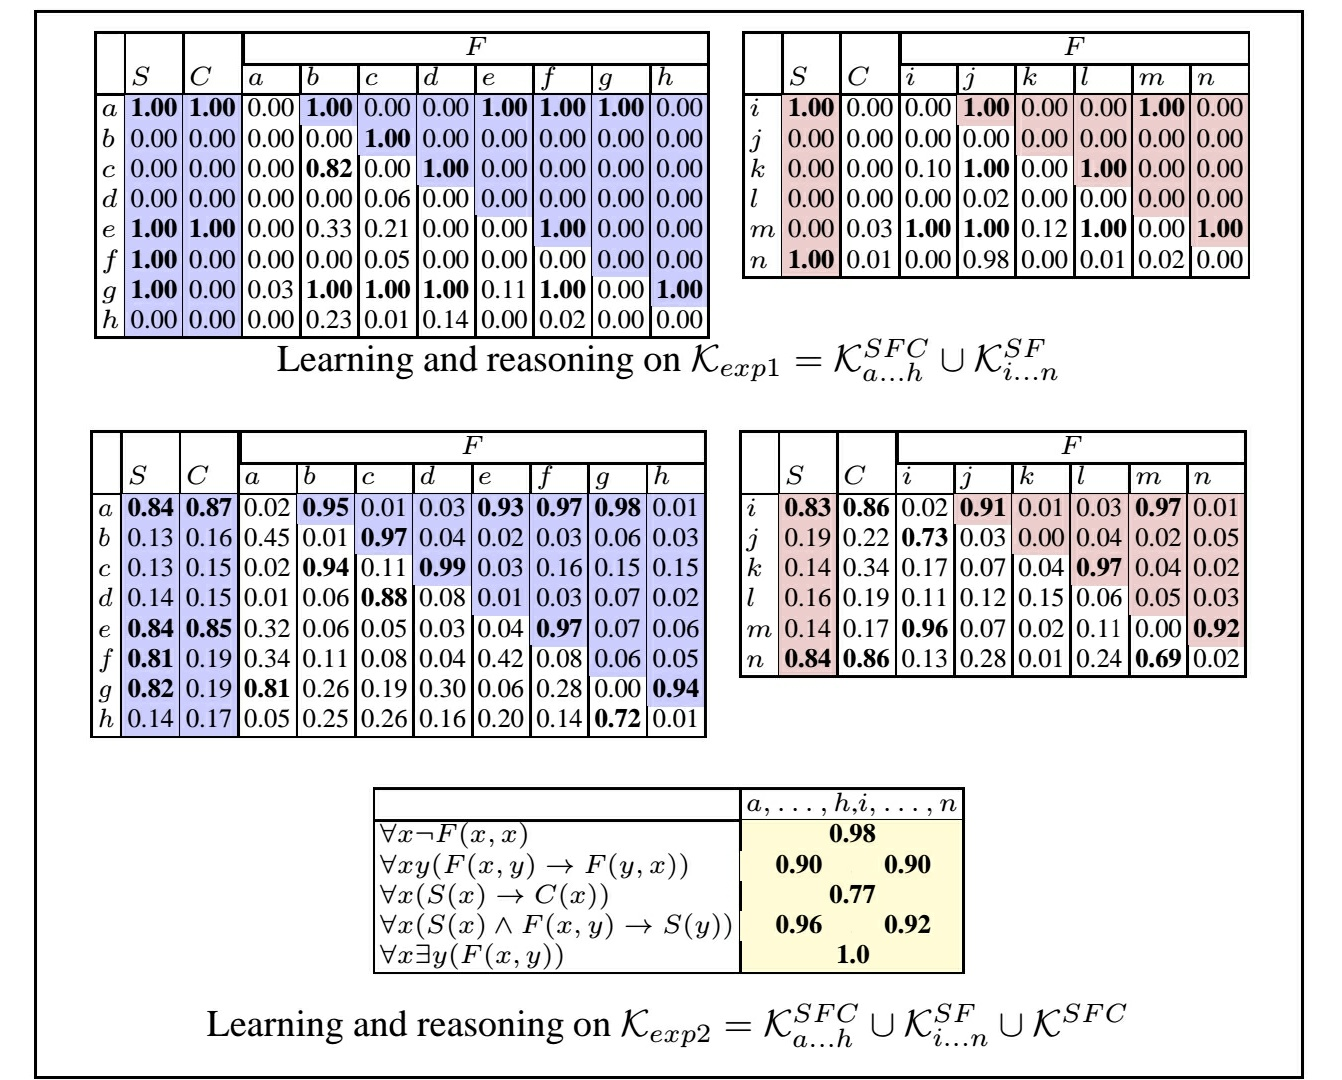
\includegraphics[scale=0.2]{table}
	\caption{Knowledge base completed by ``ltn'' \cite{LTN}}
\end{figure}

\section{Personal thoughts}

\subsection{Questions raised by the model}
This article raises a number of questions for the reader and it puts into perspective the human tendency to try and clone our way of thinking. This has been the essence of programming since its beginning and it has worked out so far, since the ``plan'' was to mathematically prove something before actually implementing it. This is still true, even in the field of artifficial intelligence, since we still tend to try and prove that neural networks actually work and produce the expected results. On the other hand, by trying to integrate a form of common sense into a program, is it still possible to try and deterministically (or even probabiilistically) predict what is going to happen? Moreover, is it really possible to replicate human thinking with such an abstract approach? We are trying to completely replace the chemical reactions happening in a real neural network with statistical conclusions, while completely bypassing the actual way that these conclusions are reached in reality. To make this work, reality has been projected into something more abstract, like, in this case, tables have been turned into vectors with a number of attributes, or maps have been turned into graphs. Similar to the tensor network, the human rationale cannot simply be followed, so we write the process off as what is going on in the ``hidden layers''. The issue is that even though we cannot follow the calculations made in a Logic Tensor Network, it is theoretically feasible to find out what each node does. Proof of this affirmation can be seen in the section where I present the basics of a neural network and the partial derivative - we are able to figure out exactly how much each neuron affects the end result. If we now transfer attention to the human brain, we realise that we actually have no clue of what goes on in a neuron. As a result, we try to imitate human thinking on a more abstract and simplified level than is necessary to completely replicate the process. To better visualise this issue, I propose the following example: imagine a beginner programmer writing a for loop and a seasoned programmer doing the same. One of them sees it as a simple number that iterates over the natural numbers in an interval, similar to writing a certain number of steps on a piece of paper. The experienced programmer knows it's possible that the iterator be held in a register, thus increasing efficiency and even suggest to the compiler that this be the case. In this situation, the result is not necessarily visible, but the fact of the matter is that one program is fundamentally different from the other, while on an abstract level they are identical and the end results are merely similar. 

\subsection{Possible uses for Logic Tensor Networks}
Logic Tensor Networks have been proved to be effective at knowledge base completion and software like Google Assistant and speech recognition in general seem to be a growing industry. This domain can greatly benefit from a similar model, not only for the actual recognition, but also for interpreting the registered text. For instance, one thing I noticed while trying to find out the limits of the increasingly popular Google Assistant was that, for the moment, it was limited to quite simple tasks. Giving more complex commands determined it to simply search the internet for the said text. A neural network that gives an agent the ability to infer what a user meant could greatly help the evolution of similar software. This is, ultimately, just an example, I believe that Logic Tensor Networks could also be used to interpret text, maybe even undertones in speech.

%Questions I thought of while writing
%Better presentation of first order logic

\begin{thebibliography}{9}
\bibitem{LTN}
	Luciano Serafini si Artur d'Avila Garcez - Logic Tensor Networks: Deep Learning and Logical Reasoning from Data and Knowledge
	
\bibitem{NTN}
	Richard Socher, Danqi Chen, Christopher D. Manning, Andrew Y. Ng - Reasoning with Neural Tensor Networks for Knowledge Base Completion

\bibitem{Tensor}
	Wolfram MathWorld, 28.12.2017\\
	http://mathworld.wolfram.com/Tensor.html

\bibitem{Tensor_Rank}
	Wolfram MathWorld, 28.12.2017\\
	http://mathworld.wolfram.com/TensorRank.html
	
\bibitem{Tensor_Multiplication}
	Joseph C. Kolecki - An Introduction to Tensors for Students of Physics and Engineering

\bibitem{Deep_Learning}
	Analytics Vidhya, 28.12.2017\\
	https://www.analyticsvidhya.com/blog/2016/03/introduction-deep-learning-fundamentals-neural-networks/
	
\bibitem{FOL}
	David W. Kueker - Mathematical Logic I (Course), 28.12.2017\\
	http://www-users.math.umd.edu/~dkueker/
	
\bibitem{Clause}
	Wikipedia, 28.12.2017\\
	https://en.wikipedia.org/wiki/Clause\_(logic)
	
\bibitem{Closed_Term}
	John Fremlin, 28.12.2017\\
	http://john.fremlin.de/schoolwork/logic/logic/node7.html
	
\bibitem{Free_Variable}
	Wikipedia, 28.12.2017\\
	https://en.wikipedia.org/wiki/First-order\_logic\#Free\_and\_bound\_variables

\bibitem{Atomic_Formula}
	Wikipedia, 28.12.2017\\
	https://en.wikipedia.org/wiki/Atomic\_formula
	
\bibitem{Literal}
	Wikipedia, 28.12.2017\\
	https://en.wikipedia.org/wiki/Literal\_(mathematical\_logic)

\end{thebibliography}

\end{document}